\chapter{Implementasi dan Pengujian}
\label{chap:implementasidanpengujian}
Bab ini berisi Implementasi Perangkat Lunak dan Pengujian Perangkat Lunak. Bagian implementasi terdiri dari penjelasan lingkungan pengembangan perangkat lunak dan hasil implementasi. Bagian pengujian terdiri dari hasil pengujian fungsional dan eksperimental terhadap perangkat lunak yang telah dibangun.

\section{Implementasi}
\label{sec:implementasi} 

\subsection{Lingkungan Implementasi}
Implementasi perangkat lunak ini dilakukan pada komputer penulis dengan spesifikasi berikut:
\begin{enumerate}
	\item \textit{Processor}: Intel Core i5 9400F
	\item \textit{Random Access Memory} (RAM): 16 GB DDR4
	\item Sistem Operasi: Windows 10
	\item Versi Python : Python 3.8.5
\end{enumerate}

\subsection{Hasil Implementasi}
Hasil implementasi berupa sebuah perangkat lunak perekaman kehadiran daring otomatis dengan bahasa pemrograman python. Sebelum menjalankan perangkat lunak untuk perekaman kehadiran daring otomatis, terdapat \textit{file} .ini yang merupakan sebuah masukkan untuk perangkat lunak. \textit{File} .ini dibahas pada Subbab \ref{sec:inputConfig}. Contoh \textit{file} .ini dapat dilihat pada \ref{kode:5:kodemasukan}.
\begin{lstlisting}[caption=Contoh \textit{file} .ini untuk Masukan Perangkat Lunak Perekaman Kehadiran Daring Otomatis, label=kode:5:kodemasukan]
	[database_config]
	1 = open https://studentportal.unpar.ac.id
	2 = click #login-button
	3 = sendkeys #username 2017730035@student.unpar.ac.id 
	4 = click #next_login
	5 = sendkeys #password 12345
	6 = click #appPass>div.login__form>button
	7 = or a[href='https://studentportal.unpar.ac.id/jadwal'] .swal-button.swal-button--confirm.swal-button--danger
	8 = click a[onclick="absenPerkuliahan(this)"]
	9 = click .swal-button.swal-button--confirm.swal-button--danger9
	10 = quit
\end{lstlisting}

Perekaman kehadiran daring otomatis dapat dilakukan dengan menjalankan perangkat lunak. Pengguna perlu membuka \textit{Command Prompt} pada komputer maupun laptop dengan \textit{directory} file automatedTesting.py berada dan menuliskan perintah ``python automatedTesting.py'' atau ``py automatedTesting.py'' pada \textit{Command Prompt}, seperti pada tampilan Gambar \ref{fig:cmd}
\begin{figure}[H]
	\centering
	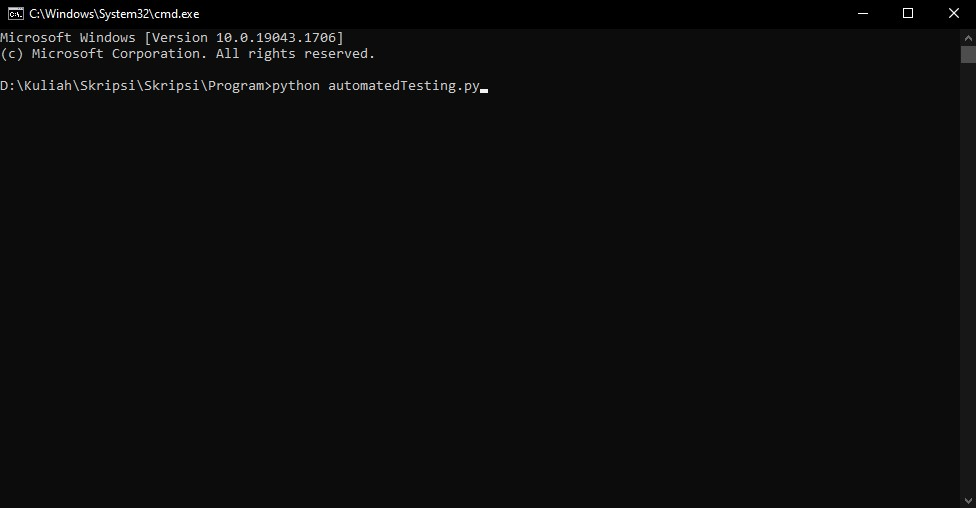
\includegraphics[scale=0.5]{Gambar/cmd.jpg}
	\caption{Tampilan \textit{Command Prompt} dengan \textit{Directory File}} 
	\label{fig:cmd}
\end{figure}

Setelah pengguna menekan ``Enter'' pada \textit{Command Prompt} maka perangkat lunak akan melakukan perekaman kehadiran daring secara otomatis, bagi mahasiswa maka perangkat lunak akan melakukan perekaman kehadiran daring pada Portal Akademik Mahasiswa secara otomatis, dimana perangkat lunak akan menjalankan secara otomatis tahap-tahap perekaman kehadiran daring secara manual yang biasa dilakukan mahasiswa seperti yang dibahas pada Subbab \ref{sec:alur}, sedangkan bagi dosen maka perangkat lunak akan melakukan perekaman kehadiran daring pada AKUHADIR seperti yang dibahas pada Subbab \ref{sec:akuhadir}. Setelah berhasil melakukan perekaman kehadiran daring maka akan muncul notifikasi bahwa perekaman berhasil dilakukan, seperti pada tampilan Gambar \ref{fig:absenBerhasil}, selain itu akan muncul notifikasi berupa peringatan bahwa absensi gagal, seperti pada tampilan Gambar \ref{fig:absenGagal}. Absensi gagal terjadi karena tidak ada jadwal kuliah lagi bagi mahasiswa, atau sudah melakukan absensi sehingga tidak ada yang bisa lagi untuk melakukan perekaman kehadiran.
\begin{figure}[H]
	\centering
	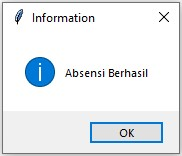
\includegraphics[scale=0.7]{Gambar/infoBox.jpg}
	\caption{Tampilan Notifikasi Berhasil Absen} 
	\label{fig:absenBerhasil}
\end{figure}

\begin{figure}[H]
	\centering
	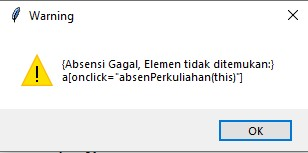
\includegraphics[scale=0.7]{Gambar/gagalAbsen.jpg}
	\caption{Tampilan Notifikasi Gagal Absen} 
	\label{fig:absenGagal}
\end{figure}

\section{Pengujian}
\label{sec:pengujian} 

\subsection{Pengujian Fungsional Mahasiswa}
Pengujian fungsional dilakukan untuk mengetahui kesesuaian reaksi perangkat lunak dengan reaksi yang diharapkan berdasarkan aksi pengguna terhadap perangkat lunak. Tabel \ref{tab:fungsi} merupakan tabel hasil pengujian perangkat lunak pada komputer penulis dengan spesifikasi berikut:
\begin{enumerate}
	\item \textit{Processor}: Intel Core i5 9400F
	\item \textit{Random Access Memory} (RAM): 16 GB DDR4
	\item Sistem Operasi: Windows 10
	\item Versi Python : Python 3.8.5
\end{enumerate}

\begin{table}[H]			
	\caption{Tabel Pengujian Fungsional}
	\centering
	\begin{tabular}{|p{0.5cm} |p{4cm} |p{5.5cm}| p{3cm}|} \hline
		No. & Aksi Pengguna & Reaksi yang diharapkan & Reaksi Perangkat Lunak\\ \hline     
		1. 	& Mahasiswa menjalankan perangkat lunak & Browser Google Chrome terbuka & Sesuai\\ \hline 
	 		& &  Browser menuju situs Portal Akademik Mahasiswa & Sesuai\\ \hline 
			& &  Browser menuju halaman web untuk perekaman kehadiran daring & Sesuai\\ \hline 
			& &  Melakukan perekaman kehadiran daring secara otomatis & Sesuai\\ \hline
	\end{tabular}
	\label{tab:fungsi}
\end{table}

\subsection{Pengujian Fungsional Dosen}

\textit{Subbab ini ditulis oleh dosen pembimbing.}

Program yang sudah dibuat diujikan juga di komputer dosen pembimbing, untuk melakukan rekam kehadiran pada portal AKUHADIR (subbab \ref{sec:akuhadir}). Berikut adalah spesifikasi komputer yang digunakan untuk menguji:

\begin{enumerate}
	\item \textit{Processor}: Intel Core i3-2120 CPU @ 3.30GHz \times 4
	\item \textit{Random Access Memory} (RAM): 6,0 GiB
	\item Sistem Operasi: Ubuntu 22.04 LTS
	\item Versi Python : Python 3.10.4
\end{enumerate}

Untuk melakukan perekaman kehadiran otomatis di AKUHADIR, perlu penyesuaian \textit{file} \texttt{database.ini} seperti dilihat pada kode \ref{kode:5:databasedosen}.

\begin{lstlisting}[caption=\textit{File} \texttt{database.ini} AKUHADIR (\textit{password} disembunyikan), label=kode:5:databasedosen]
[database_config]
1 = open https://akuhadir.unpar.ac.id
2 = sendkeys #username pascal@unpar.ac.id
3 = click #next_login
4 = sendkeys #password xxx
5 = click button[name=submit]
6 = click a[href='https://akuhadir.unpar.ac.id/absensi?tab=tab2']
7 = click a[onclick='checkin_home()']
8 = quit
\end{lstlisting}

Saat pertama kali dijalankan, program menghasilkan pesan kesalahan seperti ditunjukkan pada kode \ref{kode:5:tkintererror}.

\begin{lstlisting}[caption=Pesan kesalahan skrip tanpa \textit{tkinter}, label=kode:5:tkintererror]
$ python3 automatedTesting.py 
Traceback (most recent call last):
  File "/home/pascal/Downloads/Dosen/automatedTesting.py", line 11, in <module>
    from tkinter import * 
ModuleNotFoundError: No module named 'tkinter'
\end{lstlisting}

Dengan adanya kesalahan tersebut, dosen juga mengulangi pengujian di komputer lain, yaitu:

\begin{enumerate}
	\item \textit{Processor}: Apple M1
	\item \textit{Random Access Memory} (RAM): 8 GB
	\item Sistem Operasi: macOS Monterey
	\item Versi Python : Python 3.9.10
\end{enumerate}

Saat dijalankan, program menghasilkan pesan kesalahan yang serupa, seperti ditunjukkan pada kode \ref{kode:5:tkintererrormac}

\begin{lstlisting}[caption=Pesan kesalahan skrip tanpa \textit{tkinter}) pada komputer alternatif, label=kode:5:tkintererrormac]
 % python3 automatedTesting.py
Traceback (most recent call last):
  File "/Users/pascal/Downloads/Dosen/automatedTesting.py", line 13, in <module>
    from tkinter import * 
  File "/opt/homebrew/Cellar/python@3.9/3.9.10/Frameworks/Python.framework/Versions/3.9/lib/python3.9/tkinter/__init__.py", line 37, in <module>
    import _tkinter # If this fails your Python may not be configured for Tk
ModuleNotFoundError: No module named '_tkinter'
\end{lstlisting}

Dari pengamatan pesan kesalahan, didapatkan bahwa program ini membutuhkan pustaka lain, yaitu \texttt{tkinter}. Dalam kasus ini dosen pembimbing tidak melanjutkan \textit{troubleshooting} karena pada paket program yang dikirimkan tidak mengandung instruksi untuk melakukan instalasi pustaka tersebut. Oleh karena itu pengujian fungsional pada komputer dosen dinyatakan tidak berhasil, dan selengkapnya dapat dilihat pada tabel \ref{tab:fungsidosen}.

\begin{table}[H]			
	\caption{Tabel Pengujian Fungsional}
	\centering
	\begin{tabular}{|p{0.5cm} |p{4cm} |p{5.5cm}| p{3cm}|} \hline
		No. & Aksi Pengguna & Reaksi yang diharapkan & Reaksi Perangkat Lunak\\ \hline     
		1. & Dosen menjalankan perangkat lunak & Browser Google Chrome terbuka & Tidak sesuai\\ \hline 
		 	& &  Browser menuju situs AKUHADIR & Tidak sesuai\\ \hline
		 	& &  Browser menuju halaman web untuk perekaman kehadiran & Tidak sesuai\\ \hline
		 	& &  Melakukan perekaman kehadiran daring secara otomatis & Tidak sesuai\\ \hline
	\end{tabular}
	\label{tab:fungsidosen}
\end{table}


\subsection{Pengujian Eksperimental}
Pengujian eksperimental dilakukan terhadap beberapa mahasiswa Universitas Katolik Parahyangan jurusan Teknik Informatika yang sudah memiliki Google Chrome dan Python3. Metode pengujian dilakukan dengan cara menyebarkan perangkat lunak yang dapat diunduh melalui Google Drive. Setelah menjalankan perangkat lunak tersebut, mahasiswa diminta untuk mengisi Google Form untuk mengetahui kelancaran perangkat lunak ketika dijalankan dan mengetahui lama waktu yang dibutuhkan hingga program berhasil melakukan perekaman kehadiran. Berikut ini hasil yang didapatkan dari pengisian survei:
\begin{itemize}
	\item Dari 7 responden yang telah mengisi survei, memberi respons bahwa perangkat lunak berjalan dengan baik dan dapat melakukan perekaman kehadiran daring secara otomatis. Hasil diagram lingkaran pada Gambar \ref{fig:noerror} menunjukan bahwa semua responden menyatakan setuju program tidak mengalami \textit{error} atau \textit{crash}.
	\begin{figure}[H]
		\centering
		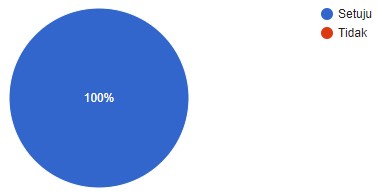
\includegraphics[scale=0.7]{Gambar/diagramLingkaran.jpg}
		\caption{Diagram Lingkaran Kesetujuan Perangkat Lunak Tidak \textit{Error} atau \textit{Crash}} 
		\label{fig:noerror}
	\end{figure}
	\item Tabel \ref{tab:otomatis} menunjukan waktu yang didapatkan dari 7 responden dalam menjalankan perangkat lunak untuk melakukan perekaman kehadiran daring otomatis. Hasil tabel tersebut menunjukan bahwa dalam melakukan perekaman kehadiran daring otomatis berada di rentang waktu 11-22 detik dan hasil rata-rata waktu adalah 16,71 detik.
	\begin{table}[ht]			
		\caption{Tabel Perekaman Kehadiran Otomatis}
		\centering
		\begin{tabular}{|p{3.5cm} |p{7cm}|}
			\hline
			Jumlah Responden &  Waktu Perekaman Kehadiran Otomatis \\ \hline     
			1 orang &  11 detik\\ \hline 
			1 orang &  14 detik\\ \hline 
			1 orang &  15 detik\\ \hline 
			2 orang &  18 detik\\ \hline 
			1 orang &  19 detik\\ \hline 
			1 orang &  22 detik\\ \hline 
		\end{tabular}
		\label{tab:otomatis}
	\end{table}
	\item Diagram lingkaran pada Gambar \ref{fig:interaksi} menunjukan bahwa sebanyak 7 responden menyatakan setuju bahwa perangkat lunak untuk melakukan perekaman kehadiran daring secara otomatis dapat membuat waktu interaksi dengan situs web atau browser menjadi lebih singkat.
	\begin{figure}[H]
		\centering
		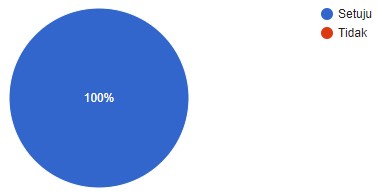
\includegraphics[scale=0.7]{Gambar/diagramLingkaran.jpg}
		\caption{Diagram Lingkaran Kesetujuan Perangkat Lunak Menghemat Waktu Interaksi dengan Browser} 
		\label{fig:interaksi}
	\end{figure}
\end{itemize}
	
